% \begin{figure}[H]
%     \centering
%      {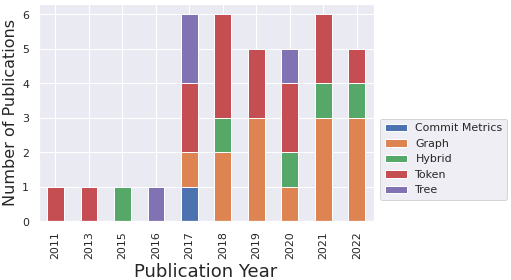
\includegraphics[width=0.6\textwidth]{Figures/RQ1/rep_by_time.png}}\
%      \vspace{-0.1in}
%      \caption{Different representation techniques distributed over time.}
%     \label{fig:rep_over_time}
% \end{figure}

\definecolor{ultrapink}{rgb}{1.0, 0.44, 1.0}
\pgfplotstableread{
Date  Commit Graph 	Hybrid 	Token 	Tree
2011 	0 	0 	0 	1 	0
2013 	0 	0 	0 	1 	0
2014	0 	0 	0 	1 	0
2015	0 	0 	1 	0 	0
2016 	0 	0 	0 	0 	1
2017 	1 	1 	0 	2 	2
2018 	0 	3 	1 	4 	1
2019 	1 	3 	0 	3 	2
2020 	0 	2 	1 	2 	1
2021 	0 	10 	2 	4 	2
2022 	1 	7 	2 	2 	2
}\testdata
\begin{figure}[t!]
\centering
\renewcommand{\arraystretch}{1}
\resizebox{0.6\columnwidth}{!}{%
    \begin{tikzpicture}[scale=0.6]
    \begin{axis}[
        ybar stacked,
    	bar width=15pt,
        ymin=0,
        ymax=20,
        xtick=data,
        legend style={at={(1.01,0.54)},anchor=west},
        reverse legend=true,
        %yticklabels from table={\testdata}{Label},
        xticklabels={ {2011}, {2013}, {2014}, {2015}, {2016}, {2017}, {2018}, {2019},
       {2020}, {2021}, {2022}},
        xticklabel style={rotate=25,anchor=east},
    ]
    \addplot + [ nodes near coords, fill=green!80]      table    [y=Commit, meta=Date, x expr=\coordindex] {\testdata};
    \addplot + [ nodes near coords, fill=cyan!80]      table    [y=Graph, meta=Date, x expr=\coordindex] {\testdata};
    \addplot + [nodes near coords, fill=blue!60]         table    [y=Hybrid, meta=Date, x expr=\coordindex] {\testdata};
    \addplot + [nodes near coords, fill=red!60]         table    [y=Token, meta=Date, x expr=\coordindex] {\testdata};
    \addplot + [nodes near coords, fill=ultrapink!60] table    [y=Tree, meta=Date, x expr=\coordindex] {\testdata};
\legend{Commits,
Graph,
Hybrid,
Token,
Tree
}
\end{axis}
\end{tikzpicture}}
\caption{Distribution of data type representations in software vulnerability detection studies over time.}
\label{typeDist}
\end{figure}

